\chapter{Nakład pracy}

Rozdział opisuje wkład i zadania poczynione przez każdego członka zespołu, które zostały wykonane w celu ukończenia projektu.
Pierwszy semestr był poświęcony na wypełnianiu dokumentacji, określeniu wymagań i tworzeniu mockupów aplikacji w celu wypracowania
wspólnej wizji projektu. W drugim semestrze zespół zajmował się implementacją aplikacji.

\indent Wykres przedstawiający czas jaki członkowie zespołu spędzili nad projektem

\begin{figure}[H]
    \centering
    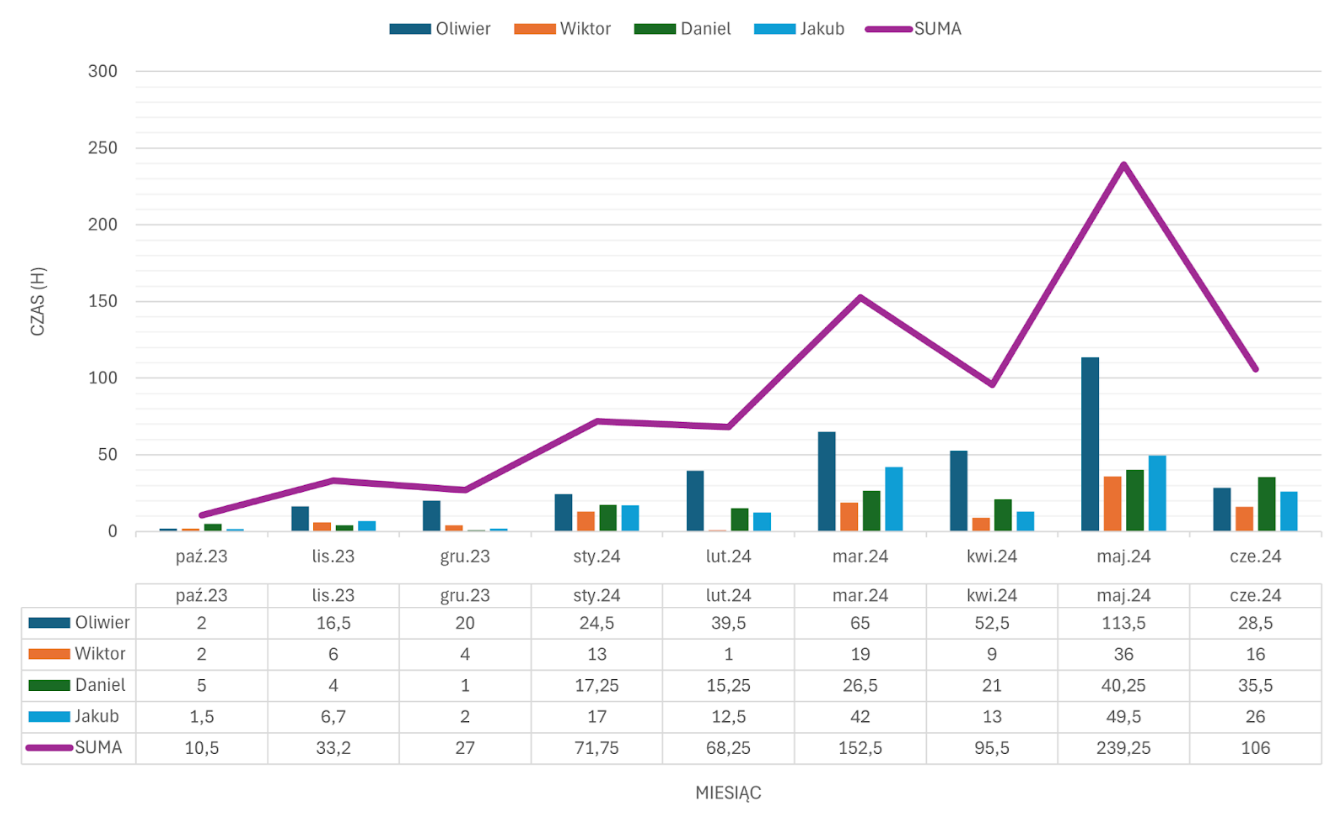
\includegraphics[width=1\textwidth]{chapters/chapter_12/naklad_pracy_wykres}
    \caption{Wykres nakładu pracy.}
    \label{img:wykres_nakładu_pracy}
\end{figure}

\subsection{Oliwier Kossak}

Na początku 1 semestru pisania pracy zająłem się wypełnieniem dokumentu założeń wstępnych.
Rozdziału dokumenty, które zostały przeze mnie napisane to analiza konkurencji, zakres systemu i wymagania jakościowe.
Następnie zająłem się wypełnianiem wymagań w specyfikacji wymagań wstępnych.
Gdy wymagania funkcjonalne zostały określone zacząłem tworzyć w canvie atrapę aplikacji mobilnej.
Kreowanie atrapy pozwoliło na konsolidację informacji i na ponownę analizę niektórych wymagań.
Byłem też osobą odpowiedzialną za konsultowanie naszych wymagań i rozwiązań z promotorem, co czyniło mnie w pewnym
sensie team leadera.
\par W drugim semestrze pisania pracy byłem odpowiedzialny za backend, frontend, testy i pisanie pracy
inżynierskiej. Przy pisaniu backendu byłem odpowiedzialny za implementację modeli fiszek, talii, i zgłoszeń.
Po utworzeniu modeli zabrałem się za napisanie do nich metod CRUD.
Moim zadaniem było także utworzenie rozwiązań związanych ze sztuczną inteligencją w naszej aplikacji.
Na początku zająłem się komunikacją z chatem gpt. Napisałem metodę post, która pozwalała na wysłanie zapytania do chatu.
Następnie zająłem się implementacją modelu nlp, który służył do wyszukiwania komendy najbardziej zbliżonej semantycznie
do tego co powiedział użytkownik podczas korzystania z trybu sterowania głosem. Do moich zadań związanych z
implementacją strony webowej należało utworzenie następujących widoków:
\begin{itemize}
    \item Strona domowa;
    \item Ranking użytkowników i talii;
    \item Panel moderatora;
    \item My decks;
    \item Public decks;
    \item Tryb uczenia się;
    \item Create deck;
    \item Voice control i memorized i not memorized flashcards.
\end{itemize}

Zaimplementowane przez mnie funkcjonalności na stronie internetowej to:

\begin{itemize}
    \item Importowanie talii;
    \item Tryb uczenia się;
    \item Tryb sterowania głosem;
    \item Generowanie treści przy użyciu chatu GPT;
    \item Wylogowanie się użytkownika;
    \item Tworzenie talii fiszek;
    \item Edycja talii;
    \item Usunięcie talii;
    \item Syntezator mowy.
\end{itemize}

Byłem też osobą odpowiedzialną za wykonywanie testów.
Gdy, któryś z członków zespołu dodawał nowy widok lub funkcjonalność do aplikacji wykonywałem
testy akceptacyjne w celu sprawdzenia czy nowy element aplikacji zachowywał się zgodnie z
oczekiwaniami. Oprócz testów akceptacyjnych wykonałem także testy integracyjne w celu
sprawdzenia czy endpointy komunikują się z bazą danych. W książce napisałem poniższe rozdziały:


\begin{itemize}
    \item 3.3 Grupa docelowa;
    \item 3.4 Analiza rozwiązań konkurencji ;
    \item 3.5 Analiza szans oraz zalet względem konkurencyjnych rozwiązań;
    \item 3.6 Analiza ryzyka;
    \item 3.7 Społeczny aspekt projektu;
    \item 7.1 Faza planowania;
    \item 7.2 Faza implementacji;
    \item Opisy sprintów w rozdziale 7;
    \item Szczegóły implementacji w rozdziale 7;
    \item Rozdział 8;
    \item Rozdział 10;
    \item Rozdział 11;
    \item Bibliografia.
\end{itemize}

\subsection{Wiktor Krieger}

W czasie semestru zimowego, oprócz pomocy przy wypełnianiu dokumentacji, zająłem się wstępną konfiguracją projektu w
serwisie Jira. Ponadto podjąłem się praktycznej analizy konkurencji, testując aplikację z rozwiązaniami zbliżonymi do
tych, które planowaliśmy zaimplementować w naszym produkcie. Testy te obejmowały ocenę użyteczności, funkcjonalności oraz
interfejsu użytkownika konkurencyjnych aplikacji, co dostarczyło nam cennych informacji pomocnych w ulepszaniu naszego
produktu. Równocześnie pomagałem przy wyszukiwaniu prac naukowych dotyczących społecznych aspektów naszego rozwiązania.
Na wczesnym etapie projektu stworzyłem również logo, które miało subtelnie sugerować, co oferuje nasz produkt.
Logo przedstawia duszka (asystenta AI) pod postacią mikrofonu (funkcje głosowe) otoczonego kolorowymi kartami (fiszkami).
Proces tworzenia logo był dla mnie szczególnie ważny, ponieważ zależało mi, aby było ono nie tylko estetyczne,
ale również intuicyjnie komunikowało funkcje naszego produktu. Natomiast większość czasu w tamtym okresie poświęciłem
na projektowaniu warstwy wizualnej aplikacji w Canvie, co pomogło w stworzeniu wspólnej wizji projektu i zostało
wykorzystane jako wzór dla finalnego produktu.
\par W kolejnym semestrze byłem odpowiedzialny za wizualne aspekty aplikacji. Moje zadania obejmowały projektowanie
tła, dobór palety kolorów oraz tworzenie ikon. Dbałem o to, aby wszystkie te elementy były spójne i estetyczne.
W części programistycznej zajmowałem się frontendem i częściowo backendem widoków aplikacji webowej, poświęcając
najwięcej pracy na ekran profilu. Moje zadania związane z implementacją strony webowej obejmowały utworzenie
następujących widoków:

\begin{itemize}
    \item Rejestracja;
    \item Logowanie;
    \item Profil;
    \item Widok statystyk.
\end{itemize}

Zaimplementowane przez mnie funkcjonalności na stronie internetowej to:

\begin{itemize}
    \item Rejestracja i logowanie;
    \item Wybór Awatara;
    \item Zmiana danych;
    \item Wyświetlanie statystyk;
    \item Usuwanie konta;
    \item Przejście do panelu moderatora dostępne tylko dla wybranych kont;
    \item Obsługa błędów w formularzach.
\end{itemize}

Aby zwizualizować nasz indywidualny wkład wykorzystałem dane zbierane przez cały czas pracy nad projektem i
dostosowałem je tak aby stworzyć czytelny wykres widoczny na początku tego rozdziału.
Oprócz tego w książce napisałem poniższe rozdziały:

\begin{itemize}
    \item 7.3.1.2 Rejestracja (web)
    \item 7.3.2.2 Logowanie (web)
    \item 7.3.4.3 Edycja danych użytkownika (web)
    \item 7.3.5.3 Usuwanie konta (web)
    \item 11.2 Porzucone pomysły (aktywacja konta i reset hasła)
\end{itemize}

\subsection{Jakub Żurawski}

W pierwszym semestrze, od momentu rozpoczętych prac nad projektem, byłem głównie odpowiedzialny za diagramy oraz część
dokumentu założeń wstępnych i część dokumentu specyfikacji wymagań technicznych. W dokumencie założeń wstępnych byłem
odpowiedzialny za rozdziały takie jakie opis problemu, cele systemu i kontekst systemu. Z kolei w dokumencie
specyfikacji wymagań systemowych byłem odpowiedzialny za wymagania ogólne i dziedzinowe, wymagania pozafunkcjonalne
oraz wymagania na środowisko docelowe. Po ukończeniu wyżej opisanych rozdziałów, przystąpiłem to tworzenie diagramu
przypadków użycia. Początkowo zakładałem, że pierwszy lepszy program wystarczy do tego, niestety później stwierdziliśmy,
że jednak przerzucenie diagramu do Enterprise Architect najlepiej prezentuje się utworzony diagram i jest najbardziej
czytelny.
\par W drugim semestrze, po podziale zespołu według zakresu pracy, byłem odpowiedzialny za backend, aplikację
mobilną oraz pisanie pracy inżynierskiej. W backendzie byłem odpowiedzialny głównie za bezpieczeństwo api, autoryzację
użytkownika oraz zarządzanie użytkownikami, np. możliwość edycji danych i usuwanie użytkowników z systemu.
Miałem również zajmować się rozwiązaniem sztucznej inteligencji w naszej aplikacji, jednak problemy napotkane podczas
tworzenia aplikacji mobilnej uniemożliwiły mi pełnienie tej roli. W początkowej fazie pisania, skupiłem się głównie na
autoryzacji. Zacząłem od utworzenia modeli bazy danych dla tokenów, zużytych tokenów i użytkownika. Następnie
utworzyłem dependencje do dekodowania tokenu użytkownika i weryfikacji jego ważności. Następnie zabrałem się tworzenie
kolejnej dependencji “RoleAccessChecker”, która jak nazwa wskazuje miała sprawdzać rolę użytkownika i blokować dostęp
użytkownikom bez uprawnień.Kolejnym krokiem było zabezpieczeniem api przed nieautoryzowanym aplikacjami, adresami czy
headerami. W tym celu utworzyłem customowe middleware’y. Do middleware’ów dodałem również sprawdzanie czy token
użytkownika nie znajduję sie tabeli zużytych tokenów. Gdy bezpieczeństwo było już gotowe, zająłem się tworzeniem
widoków do autoryzacji i użytkowników, w celu przetestowania bezpieczeństwa, funkcjonalności i poprawy błędów.
Po zaimplementowaniu wstępnych fukcjonalności na backendzie, zająłem się aplikacja mobilną, gdzię odpowiedzialny byłem
za weryfikacje czy użytkownik jest zalogowany, a także utworzeniu następujących paneli i widoków jak:

\begin{itemize}
    \item Panel użytkownika;
    \item Panel moderatora;
    \item Panel rankingu i publicznych deck’ów;
    \item Widok uczenia z obsługą głosu.
\end{itemize}

Dodatkowo byłem odpowiedzialny za animację np. Loadera, który pokazuję się podczas czytania danych.
Z zaimplementowanych funkcjonalności w aplikacji mogę wymienić:

\begin{itemize}
    \item Weryfikacja czy użytkownik jest zalogowany;
    \item Metoda ‘request’ która została użyta w wielkości serwisach;
    \item Przeglądanie rankingu i udostępnionych deck’ów razem z możliwościa filtrowania po słowach kluczowych;
    \item Ograniczenie ilości zaciąganych danych z api;
    \item Wylogowywanie użytkownika;
    \item Edycja danych użytkownika;
    \item Usuwanie konta;
    \item Potwierdzanie zmian hasłem;
    \item Usuwanie zgłoszeń i użytkowników;
    \item Sterowanie głosem podczas nauki.
\end{itemize}

Podczas pisania książki byłem odpowiedzialny za rozdziały:

\begin{itemize}
    \item Rozdział 4;
    \item Rozdział 7;
    \item Rozdział 11;
    \item Implementacja w LaTeX.
\end{itemize}

\subsection{Daniel Klimowski}

W pierwszym semestrze realizacji projektu inżynierskiego prace skupiły się początkowo na fazie planowania oraz
definicji wymagań i założeń w dokumentacji DZW i SWS. W dokumencie założeń wstępnych zredagowałem początkowo punkty
od 1. do 8. tj. “Opis problemu”, “Cele systemu”, opis sekcji “Kontekst systemu”, “Zakres systemu (funkcjonalności)”,
“Wymagania jakościowe i inne”, “Wizja konstrukcyjna” i “Ograniczenia”. Które później były uzupełniane i modyfikowane
przeze mnie oraz zespół projektowy. Tak samo podjąłem się zredagowaniu części opisowej w dokumencie specyfikacji
wymagań systemowych. Mniej więcej w tym samym czasie należało zdefiniować swój zakres obowiązków w projekcie,
zdecydowałem się wybrać implementacje infrastruktury serwerowej, wspólnie z Jakubem implementację aplikacji mobilnej
oraz nadzorować kod niniejszej pracy implementowany w LaTeX. W fazie projektowania wykonałem dodatkowo min. draft
projektu w LateX, diagram architektury oraz zainicjowałem początkowy projekt aplikacji mobilnej. Pod koniec pierwszego
semestru prac spędziłem dużo czasu na nauce języka JavaScript oraz frameworku React Native. Z tymi dwiema technologiami
nie miałem okazji pracować wcześniej. Na potrzebny projektu zrealizowałem kurs na który przeznaczyłem ok. 26 godzin.

\par Drugi semestr realizowania projektu zaczął się od intensywnych prac związanych z rozwojem aplikacji mobilnej oraz
redagowaniem niniejszej książki. W momencie w którym zarówno backend jak i aplikacja webowa i mobilna były już
funkcjonalne w znacznym stopniu, podszedłem do implementacji infrastruktury serwerowej. Opis działań rozdzielę poniżej
w tych trzech obszarach:


\textbf{Aplikacja mobilna:}

\begin{itemize}
    \item Widoki logowania, rejestracji oraz zapomniałem hasła (bez łączenia z API);
    \item Widok ekranu głównego;
    \item Widok “My decks” z funkcjonalnościami wyboru i wyszukiwania talii;
    \item Widok “My downloaded decks” z funkcjonalnościami wyboru i wyszukiwania pobranych talii;
    \item Widok “Create new deck” z funkcjonalnościami tworzenia nowej talii;
    \item Widok “Display Deck” z funkcjonalnościami podglądu decku oraz szeregiem opcji;
    \item Widok “Display Flashcards” z funkcjonalnościami podglądu, tworzenia, edycji i usuwania fiszek z talii;
    \item Widok “Create Flashcard” z funkcjonalnościami tworzenia nowych fiszek i generowania treści przy pomocy ChatGPT;
    \item Widok “Edit Flashcard” z funkcjonalnością edytowania istniejących fiszek i generowania treści przy pomocy ChatGPT;
    \item Widok “Learning Mode” oferujący tryb nauki;
    \item Widok “Memorized Flashcards” i “Unmemorized Flashcards” wyświetlający fiszki oznaczone jako przyswojone i nieprzyswojone z możliwością odsłuchu treści;
    \item Widok ‘Deck Settings” z funkcjonalnościami upublicznienia/ukrycia talii, usunięcia talii, zrestartowania talii oraz edycji talii;
    \item Widok “Display Public Deck” z funkcjonalnościami podglądu, pobrania i zgłoszenia publicznej talii.
\end{itemize}

\textbf{Serwer:}

\begin{itemize}
    \item Zainicjowanie maszyny wirtualnej z systemem Ubuntu 20.04 w platformie Azure;
    \item Konfiguracja sieci w platformie Azure;
    \item Implementacja aplikacji webowej, api oraz kontenera bazy danych na serwerze;
    \item Konfiguracja generalna i sieciowa serwera;
    \item Zakup, wygenerowanie i implementacja tokenu ChatGPT na potrzeby funkcjonalności API i aplikacji.
\end{itemize}

\textbf{Książka:}

\begin{itemize}
    \item Wstęp;
    \item Rozdział I;
    \item Rozdział II;
    \item Rozdział III sekcja 3.1 i sekcja 3.2;
    \item Rozdział V;
    \item Rozdział VI - uzupełnienie;
    \item Rozdział VII - uzupełnienie;
    \item Rozdział IX - uzupełnienie;
    \item Generalne poprawki tekstu;
    \item Implementacja w LaTeX.
\end{itemize}


